% This must be in the first 5 lines to tell arXiv to use pdfLaTeX, which is strongly recommended.
\pdfoutput=1

\documentclass[11pt]{article}

% Remove the "review" option to generate the final version.
%\usepackage[review]{acl}
\usepackage[]{acl}

\usepackage{times}

\usepackage{latexsym}

\usepackage{etoolbox}% <-- for robustify bold fonts in S columns
% \newrobustcmd\ubold{\DeclareFontSeriesDefault[rm]{bf}{b}\bfseries}% <-- changed
\robustify\bfseries

\usepackage{siunitx}
\sisetup{
    round-mode=places,
    round-precision=1,
    detect-weight=true,
    %detect-inline-weight=math,
    detect-all=true,
    table-format=2.1
}

\usepackage{booktabs}
\usepackage{multicol}
\usepackage{amssymb}
\usepackage{pifont}
\usepackage{xcolor} 
\usepackage{soul}
\usepackage{stfloats}

% For proper rendering and hyphenation of words containing Latin characters (including in bib files)
\usepackage[T1]{fontenc}
% For Vietnamese characters
% \usepackage[T5]{fontenc}
% See https://www.latex-project.org/help/documentation/encguide.pdf for other character sets

% This assumes your files are encoded as UTF8
\usepackage[utf8]{inputenc}

% This is not strictly necessary, and may be commented out,
% but it will improve the layout of the manuscript,
% and will typically save some space.
\usepackage{microtype}
\usepackage{graphicx}
\usepackage{amsmath}
\usepackage[export]{adjustbox}
\usepackage{multirow}
\usepackage{caption}
\usepackage{subcaption}
\usepackage{placeins}

\begin{document}


\newcommand{\sys}{SYS}
\newcommand{\cmark}{\ding{51}}%
\newcommand{\xmark}{\ding{55}}%
\newcounter{srCounter}
\newif\ifsrvar
\srvartrue
%\trvarfalse
\ifsrvar
\newcommand{\seb}[1]{{\small \color{red} \refstepcounter{srCounter}\textsf{[SR]$_{\arabic{srCounter}}$:{#1}}}}
\else
\newcommand{\seb}[1]{}
\fi

\newcounter{fpCounter}
\newif\iffpvar
\fpvartrue
%\trvarfalse
\iffpvar
\newcommand{\fabio}[1]{{\small \color{blue} \refstepcounter{fpCounter}\textsf{[FP]$_{\arabic{fpCounter}}$:{#1}}}}
\else
\newcommand{\fabio}[1]{}
\fi

\newcounter{mbCounter}
\newif\ifmbvar
\mbvartrue
%\mbvarfalse
\ifmbvar
\newcommand{\michele}[1]{{\small \color{purple} \refstepcounter{mbCounter}\textsf{[MB]$_{\arabic{mbCounter}}$:{#1}}}}
\else
\newcommand{\michele}[1]{}
\fi

\newcounter{syCounter}
\newif\ifsyvar
\syvartrue
%\trvarfalse
\ifsyvar
\newcommand{\scott}[1]{{\small \color{violet} \refstepcounter{syCounter}\textsf{[SY]$_{\arabic{syCounter}}$:{#1}}}}
\else
\newcommand{\scott}[1]{}
\fi

\newcounter{plCounter}
\newif\ifplvar
\plvartrue
%\plvarfalse
\ifplvar
\newcommand{\patrick}[1]{{\small \color{green} \refstepcounter{plCounter}\textsf{[PL]$_{\arabic{plCounter}}$:{#1}}}}
\else
\newcommand{\patrick}[1]{}
\fi

\newcounter{goCounter}
\newif\ifplvar
\plvartrue
%\plvarfalse
\ifplvar
\newcommand{\giuseppe}[1]{{\small \color{brown} \refstepcounter{goCounter}\textsf{[GO]$_{\arabic{goCounter}}$:{#1}}}}
\else
\newcommand{\giuseppe}[1]{}
\fi

%\iftrue
\iffalse
\renewcommand{\fabio}[1]{}
\renewcommand{\seb}[1]{}
\renewcommand{\piktus}[1]{}
\renewcommand{\michele}[1]{}
\renewcommand{\patrick}[1]{}
\renewcommand{\angela}[1]{}
\renewcommand{\jt}[1]{}
\renewcommand{\scott}[1]{}
\renewcommand{\giuseppe}[1]{}
\fi

\newcommand{\citetodo}[1]{{\color{red}(#1)}}
% If the title and author information does not fit in the area allocated, uncomment the following
%
%\setlength\titlebox{<dim>}
%
% and set <dim> to something 5cm or larger.

\newcommand{\eg}{\textit{e.g.}}  %examples{e.g.}} newcommand is used to define a new command
\newcommand{\ie}{\textit{i.e.}}  %another words
\newcommand{\system}{\textsc{RHR}}  %this means that the command system is AHR

\title{Reader Help Rerank:\\ Rerank Document for Open-Domain Question Answering}

\newcommand{\sapienza}{$^1$}
\newcommand{\sapienzafair}{$^{1,2}$}
\newcommand{\fair}{$^2$}
\newcommand{\uclfair}{$^{2,3}$}
\newcommand{\ucl}{$^3$}

\author{
Hao Xiong \\
Soochow University \\ 
libraxionghao@gmail.com}

% \robustify\bfseries
\maketitle
% \begin{abstract}
% With the development of retriever in Open-Domain Question Answering (ODQA), the performance of Question Answering (QA) is improved.In order to enhance the ability of Sparse Retriever, we propose a reranker model to rerank the retrieved passages.In this way, we can reduce the choice of wrong passages and predict the right orders of golden passages to get a better results.Compared with conversational methods, such as BM25, we conduct experiments on NQ dataset and Trivia dataset,and  improving the top-10 accuracy in retriever stage in 10 points, and 6 points accuracy improved in QA. Code and pre-trained models at \url{https://github.com/facebookresearch/rerank}.

% \end{abstract}

% \begin{figure*}[ht!]
%     \centering
%     \resizebox{\textwidth}{!}{%
%     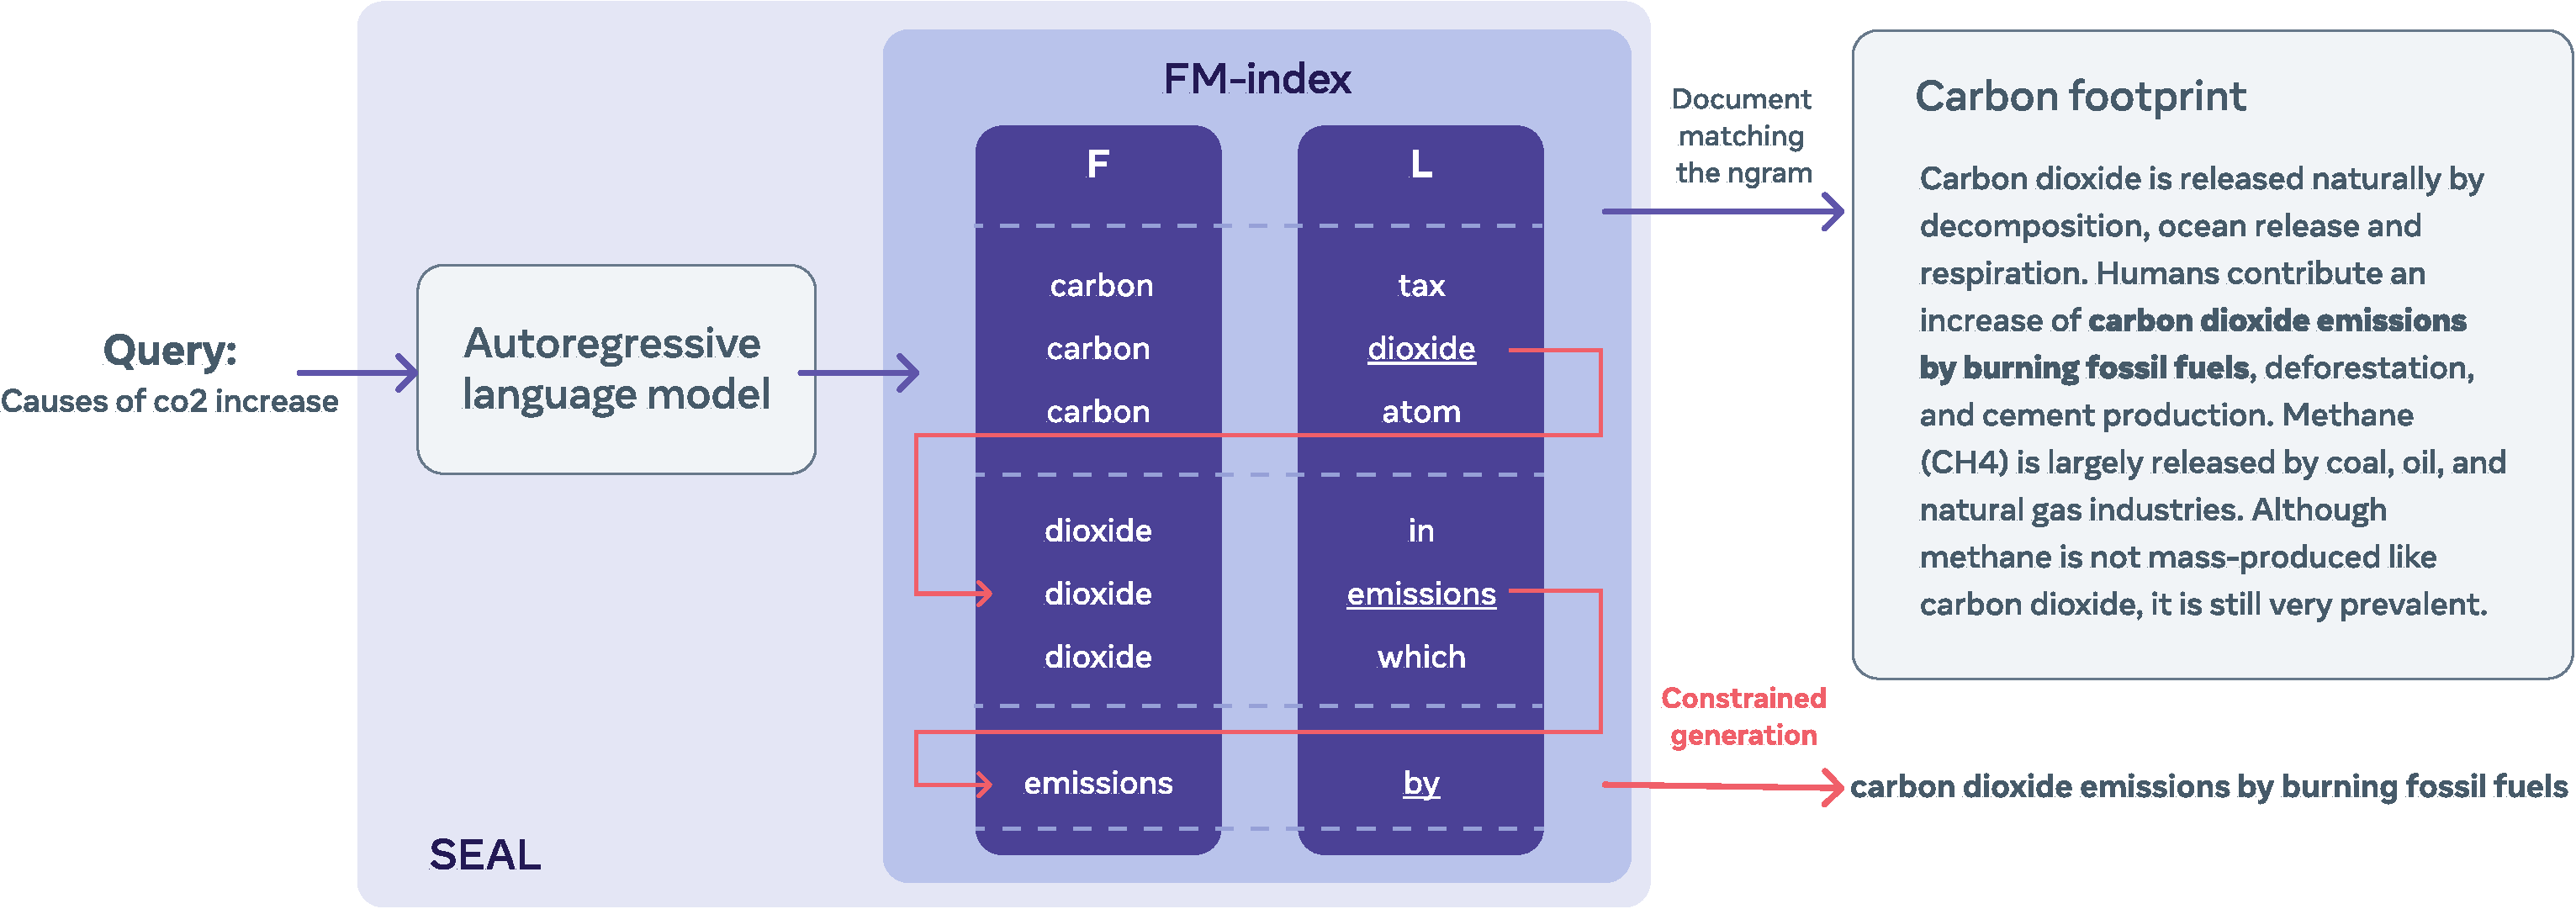
\includegraphics[
%     trim={0cm 0cm 0cm 0cm},    
%     clip=true
%     ]{figures/architecture.pdf}}
%     \caption{
%     High-level SEAL architecture, composed of an autoregressive LM paired with an FM-Index, for which we show the first (F) and last (L) columns of the underlying matrix (more details in Sec \ref{sec:fm-index}). The FM-index constraints the autoregressive generation (\eg, after \textit{carbon} the model is contrained to generate either \textit{tax}, \textit{dioxide} or \textit{atom} in the example) and provides the documents matching (\ie, containing) the generated ngram (at each decoding step).
%     }
%     \label{fig:main}
% \end{figure*}

\section{Introduction}

%here is my work
Open-Domain Question Answering (QA) is a task that aims to answer the factoid questions with amounts of documents. Previous QA systems \cite{chen2017reading} often consist of multiple components, including retriever and reader. The retriever first retrieves a small subset of the documents using the question as a query, and the reader utilize the retrieved documents as input to extract or generate the answer. 

For the purpose of enhancing the ability of the QA system, we can improve the performance of the retriever by reranking the retrieval results. Previous work \cite{karpukhin2020dense} shows that better performance in QA system can be achieved when the retrieval results are improved. Rerank the retrieval results by reranker which is a very useful approach and is wildly used after retrieval stage.

However, one limitation of the Retriever-Reranker-Reader architecture (R3) is the reranker. Conventional reranker always rerank the retrieved documents directly, it is suboptimal. Previous work  based on BERT \cite{nogueira2019passage, gao2021rethink}, rerank the retrieval documents through the questions and documents relevance. RIDER \cite{mao2021rider}  use the reader answer to rerank the documents, while it is instable.Current mainly based on seq2seq model \cite{sachan2022improving}, but is often spend much resource and time to train and inference. Therefore, we combine the answer generated by reader and the rerank model that need less resource.


%提出自己的模型
In this paper, we propose a novel Reader Help Rerank model, \system{}, which promote the QA system performance. We concatenate the question, document and answer, inputing to the \system{}, and then train the model for calculating the relevance of the question with document. At inference time, \system{} ranks the retrieved documents with the score.

We excute experiments on the Natural Questions (NQ) \cite{kwiatkowski2019natural} and TriviaQA (Trivia) \cite{joshi2017triviaqa} datasets. \system{} outperforms the state-of-the-art OpenQA systems \citep{karpukhin2020dense,sachan2021end}, and achieves EM=50 on NQ dataset and EM=51.2 on Trivia dataset. This shows the effectiveness and generalization of our approach.

Our contributions are as follows:

1. we propose \system{} to rerank the retrieved passages and achieve 10 gains in top-1 retrieval accuracy and 3 gains in QA.

2. The \system{} not only performs well on in-domain datasets, but also works well on out-of-domain datasets, showing strong generalization ability.


% \section{Related Work}

% \paragraph{Retrieval with Identifiers} One way to approach retrieval with autoregressive models makes use of identifiers, \ie, string pointers to documents that are in some way easier to generate than the full document itself. In tasks where such data is available or relevant, such as Wikipedia-based entity linking (a form of page-level retrieval), titles have been shown to work well as identifiers~\citep{decao-etal-2021-autoregressive,de-cao-etal-2021-highly,de2022multilingual}. However, even on Wikipedia-based benchmarks, titles on their own are not well-suited for retrieval at passage-level, given they can only identify an article (that might contain several passages). In a different direction, \citet{tay-etal-2021-measuring} have used hierarchical clustering on contextualized embeddings to create identifiers for arbitrary spans of text. In contrast, in our work the identifiers are corpus string matches, which do not necessarily occur in just one document.

% \paragraph{Term Weighting}
% Virtually all modern approaches to string-matching-based sparse retrieval make use of a bag-of-words assumption, indexing documents with an \emph{inverted index}, a data structure mapping terms to documents or, more generally, locations in a corpus~\citep{robertson-zaragoza-2009-probabilistic}.
% Retrieval performance in this setting depends heavily on term-weighting schemes, with many recent works proposing sophisticated, contextualized weights for both queries, and documents\citep{dai-callan-2019-context,gao-etal-2021-coil,lin-ma-2021-unicoil,mallia-etal-2021-deepimpact,dai-callan-2020-context,bai-etal-2020-sparterm,zhao-etal-2021-sparta,formal-etal-2021-splade,formal-etal-2021-spladev2}.
% Many of these methods are also able to weigh terms that are not present in the query, addressing so-called vocabulary mismatch. In contrast, \system{} generates (and assigns scores to) ngrams of arbitrary size, using the index for both generation and retrieval. Nevertheless, this line of work is partly orthogonal to our own, as many of the proposed techniques could be used to rescore higher-order ngrams.

% \paragraph{Query/Document Expansion}
% A line of research which often involves autoregressive language models is that of document and query expansion. For example, one can augment stored documents by generating possible queries that might be answered by them~\citep{nogueira-etal-2019-doc2query,nogueira-lin-2019-docTTTTTquery}. 
% In the opposite direction, works like GAR~\citep{mao-etal-2021-generation} augment the query by predicting helpful additional terms, such as an answer, sentence containing the answer, or the title of a document where the answer may be found.
% We note that while query expansion bears a superficial resemblance with \system{}, the approaches are  conceptually distinct. 
% While query expansion methods rely on a stand-alone black-box retriever, in our work the boundary between generation and retrieval is blurred, since our identifiers are grounded passage spans. 

% \paragraph{Query Likelihood Models}
% Another connected strand of research is that of query likelihood models, which, in their latest incarnations, use autoregressive models to (re)rank passages according to the probability $P(q|p)$ of a query $q$ given the passage $p$~\citep{nogueira-dos-santos-etal-2020-beyond,zhuang-zuccon-2021-tilde,lesota-etal-2021-modern}. In our case, the autoregressive architecture models the likelihood of an ngram given the query, \ie, $P(n|q)$. 

% \paragraph{``Learning to Google''}
% Recently, language models have been shown to be able to directly generate search queries for modern web search engines either with finetuning on demonstrations~\citep{Komeili2021InternetAugmentedDG,Shuster2022LanguageMT} and human preferences~\citep{nakano-2021-webgpt} or via prompting~\citep{lazaridou-etal-2022-internet}. In our case, there is no black-box retrieval system that is queried. Rather, the white-box index determines both the generated ngrams and the search process.



\bibliography{mybib}
\bibliographystyle{acl_natbib}

\FloatBarrier

\end{document}
